\section{Introduction} The core of the tracking engine is a technique
known as the \emph{particle filter}.  The particle filter is a kind of
Bayesian filtering where one uses discrete hypotheses, also known as
\emph{particles}, to approximate continuous PDF \cite{ProbRob}.  It
builds upon the theory of \emph{Markov processes} and the \emph{hidden
Markov model}.


\begin{figure} \centering
  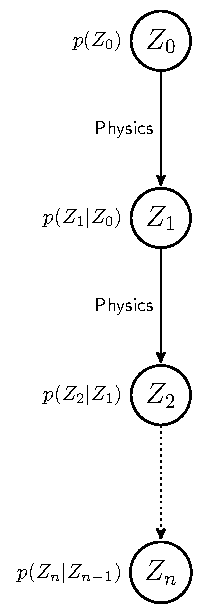
\includegraphics[width=0.175\textwidth]{mp-graph.pdf}
  \caption{Schematic image of a Markov process.}
  \label{fig:hmm-graph}
\end{figure}


\section{Markov processes} A Markov process is a special case of a
stochastic process. For a Markov process, the next state depends only
on the present state and not on past states.  For this reason, a
Markov process is often said to be ``forgetful''.

In mathematical terms, a Markov process satisfies the following:
\begin{equation} p\left(Z_t|Z_{t-1} \wedge Z_{t-2} \wedge \dots \wedge
Z_0\right) = p\left(Z_t|Z_{t-1}\right),
\end{equation} $p\left(Z_t|Z_{t-1} \wedge Z_{t-2} \wedge \dots \wedge
Z_0\right)$ is the probability that the system will have state $Z_t$
at time $t$, given that the previous states where $Z_{t-1},
Z_{t-2},\dots, Z_0$.

\begin{figure} \centering
  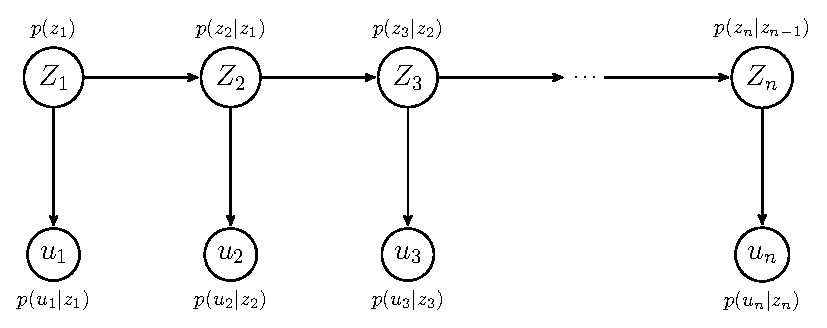
\includegraphics[width=0.35\textwidth]{hmm-graph.pdf}
  \caption{Schematic image of a hidden Markov model.}
  \label{fig:hmm-graph}
\end{figure}

<<figure of markov process only>>

\section{The Hidden Markov Model}

The working principle of the particle filter is based on the
\emph{hidden Markov model} (HMM).  A HMM describes a Markov process
where we cannot measure the state directly - it is
``hidden''\cite{EncyclopediaMachineLearning}.  Instead we obtain an
\emph{observation} $I$\footnote{In this thesis, the observation is
always a grayscale \emph{image}, therefore the observation is denoted
$I$.}  of the state. This \emph{perception} is generally
non-deterministic, so we need to denote it as $p(I_t|Z_t)$ which is
the probability that we will observe $I_t$ if the state is $Z_t$.

\section{The Curse of Dimensionality} A phenomenon that becomes
apparent in high-dimensional spaces is the so-called ``Curse of
dimensionality'' \cite{EncyclopediaMachineLearning}.  The problem is
that the search volume grows exponentially with the number of
dimensions.  It originates from the fact that we need $\Ordo{C^n}$
samples to obtain a sample density of $C$ in a $n$-dimensional space.

The first consequence of this is that in order to approximate a
high-dimensional function one needs orders of magnitude more samples.

The other drawback with high dimensional space is the large
``borders'' of the sample-set compared to lower dimensional space
which results in orders of magnitude higher chance for an point one
want to approximate to fall outside the sample-set and needs to be
extrapolated instead of the better alternative of interpolation.

% For example, consider an interval on a number line, where we cover
% the middle third of the interval with samples.  If we randomly
% select a number from the interval, there is a one in three chance
% that our selected number is in the region with samples.  Take this
% to two dimensions, and we have covered only a ninth of the space,
% and so on. This means that the chance that the point we want to
% approximate falls outside the sample set is orders of magnitude
% higher in higher dimensional spaces, compared to lower dimensional
% ones.  We need more samples in order to be able to interpolate
% between samples.

\begin{example} Figure \ref{fig:curse-of-dimensionality} shows 128
randomly scattered points in 1, 2 and 3 dimensions. Notice how the
density decreases with increasing dimension.
  \begin{figure}
    \begin{tabular}{rcl}
      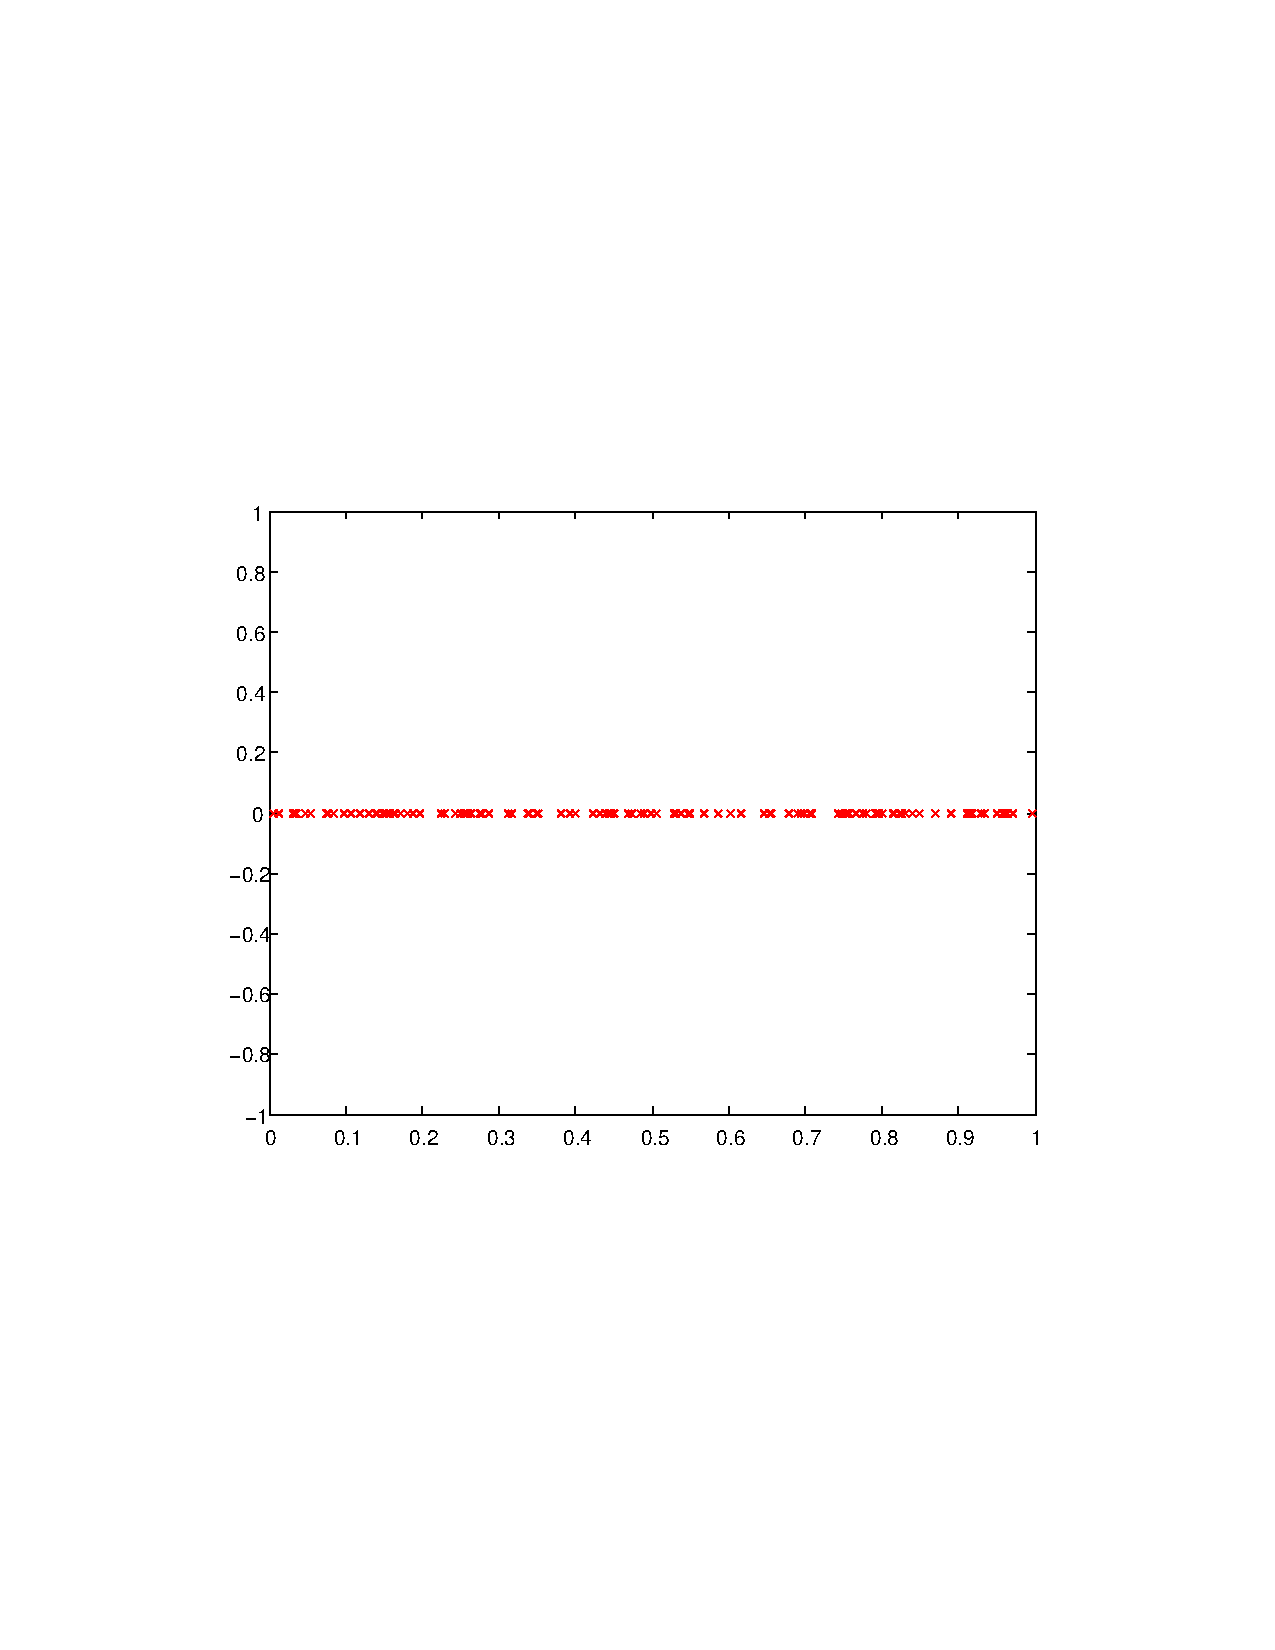
\includegraphics[scale=0.3,trim=4cm 4cm 4cm 4cm]{1D.pdf}&
      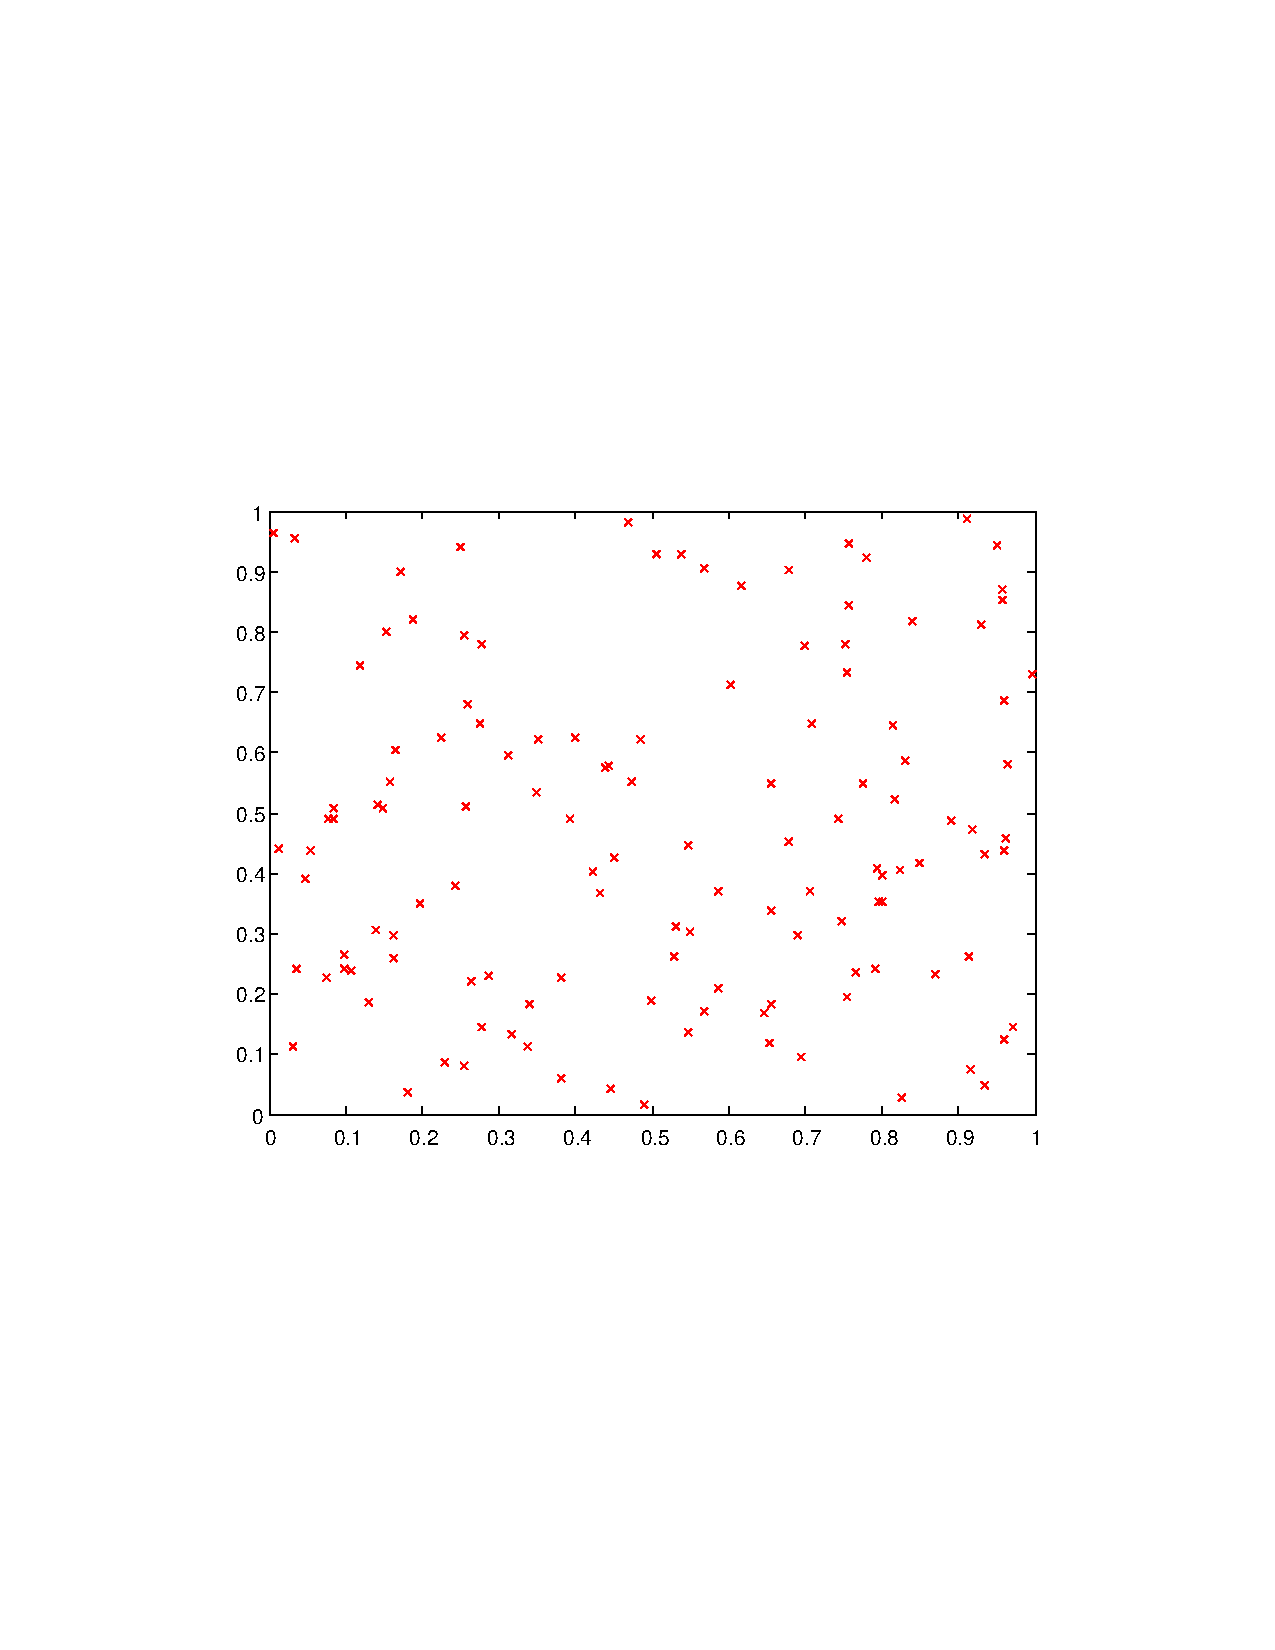
\includegraphics[scale=0.3,trim=4cm 4cm 4cm 4cm]{2D.pdf}&
      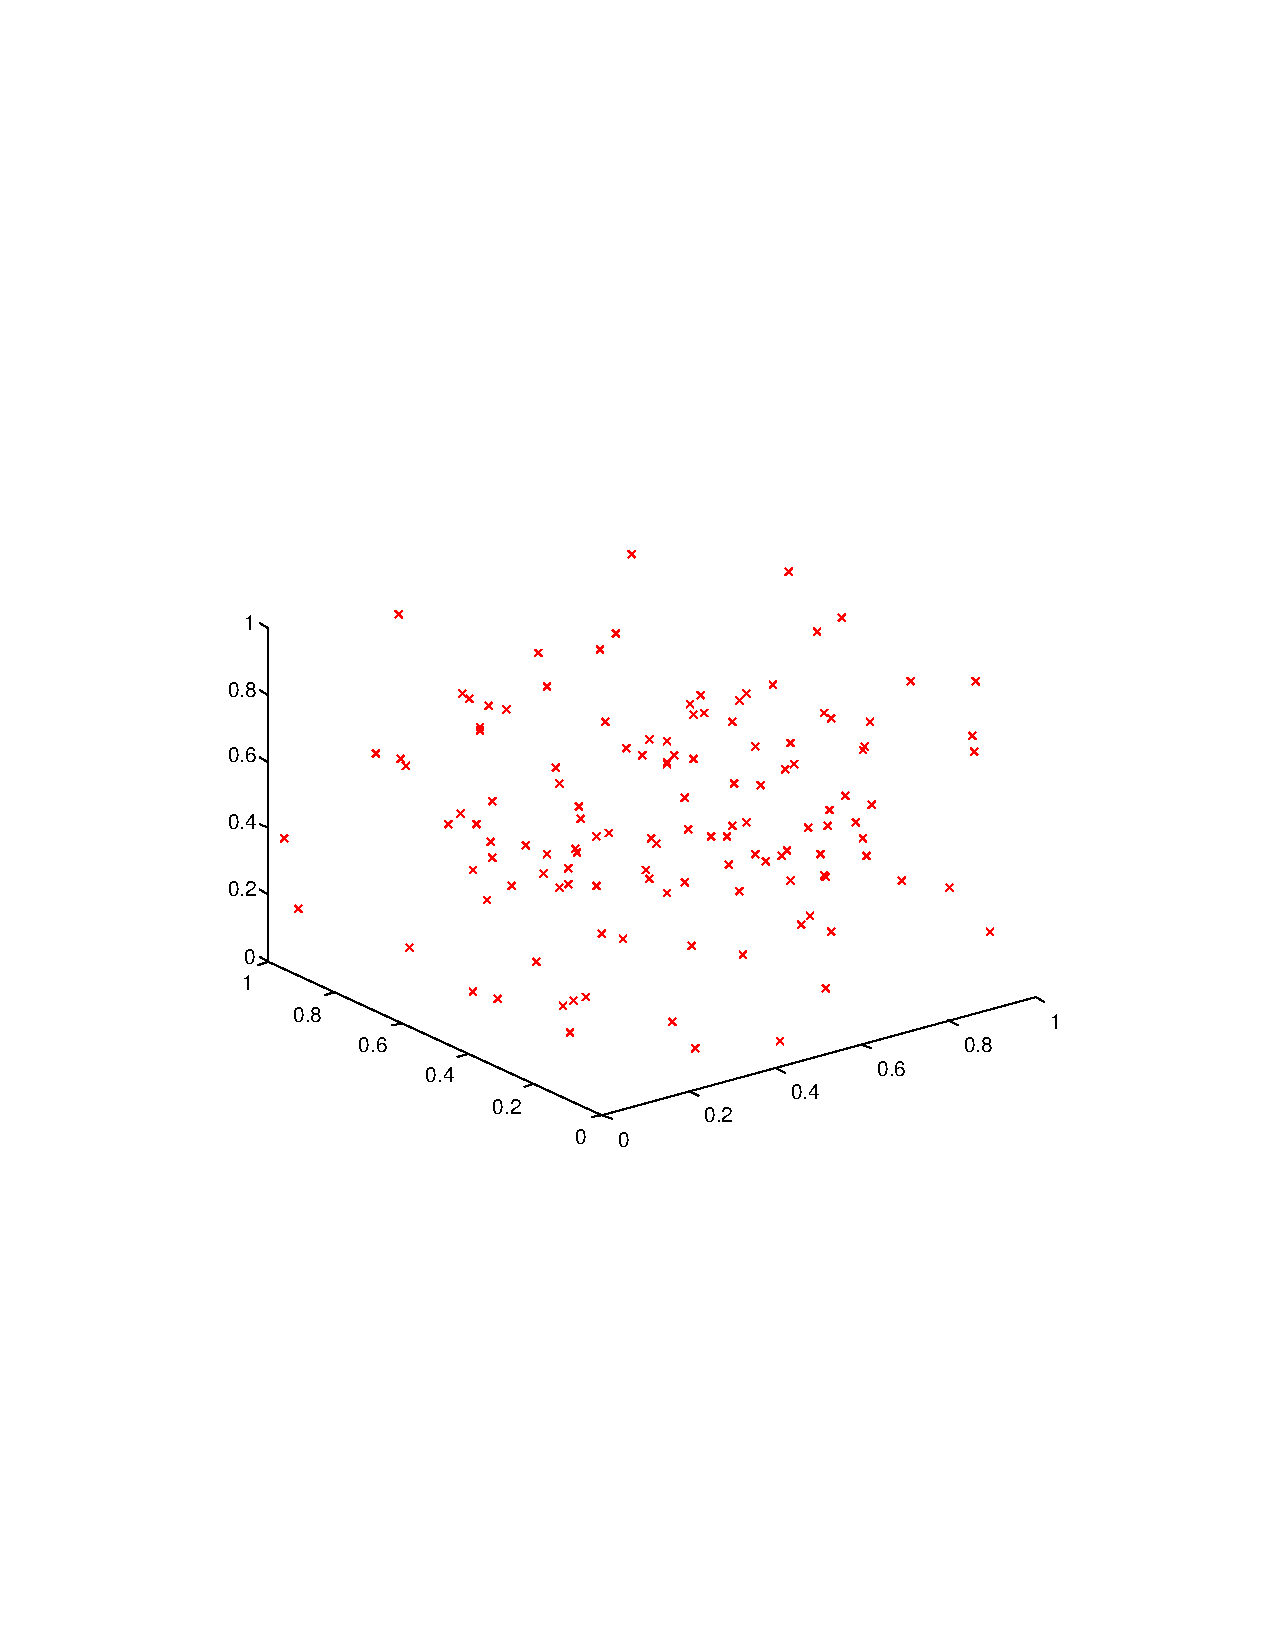
\includegraphics[scale=0.3,trim=4cm 4cm 4cm 4cm]{3D.pdf}
    \end{tabular}
    \caption{Plots of $128$ scattered samples in $1$, $2$ and $3$
dimensions, respectively.}
    \label{fig:curse-of-dimensionality}
  \end{figure}
\end{example}

\begin{example} For a $16$ DOF model one needs $10^{16}=10$
quadrillion datapoints to acquire a density of $10$ samples per unit
volume. Millions of gigabytes would be needed just to store the
samples.
\end{example}

\begin{example} In 2 dimensions it is sometimes feasible to use an
exhaustive search.  An example of this is the Hough transform
\cite{DigitalImageProcessing}, where the search is done through the
$\rho\theta$ space of line responses on images.
\end{example}

\subsection{Overcoming the Curse} One way to overcome the curse in the
context of tracking is to perform a directed search. Let the search be
in an $n$ dimensional space with a grid of $g$ grid lines in each
direction.

\begin{enumerate}
\item Use the information about the most recent\footnote{In the
    Bayesian case, the most recent estimate} location and assume that
  the tracked object cannot travel more than $R < g$ grid steps in one
  time step.  This reduces the volume of the (discrete) search space
  from $\Ordo{g^n}$ to $\Ordo{R^n}$.
      % \begin{proof}
      %   Change the coordinate system to generalized spherical
      %   coordinates $(r,\phi_1,\phi_2,...,\phi_{N-1})$ and fixate
      %   $r$ foreach $r<R$ which gives us a $(N-1)$ dimensional
      %   search surface, sum up the fixated $r$'s to get the total
      %   search space.
      % \end{proof}
\item With prior knowledge of how the tracked objects move
  \footnote{Such as the state transition probabilites $\cprobnext{Z}$
    in a HMM} we can direct our search to specific regions in the
  state space, depending on how probable it is for the tracked object
  to be located there. This reduces the size of the search space
  depending on how sure we are of the previous state.
\end{enumerate}

% This phenomen of having hue searchspace in highdimensinonal space is
% fairly common and have the name "Curse of dimensionality".

% One way to somewhat overcome this emptyness in space is to have a
% dynamic (active?) algorithm that adopts the sample density according
% to the models relative frequency in that area and this results in,
% for a given amount of samples, its more likely for an sampled model
% to occure in a more densly pre-sampled (pre-sampled?) area, in fact
% this method when doing it right (ideally) gives: given a set of
% samples the overall density for all the samples in the
% sampledatabase would be optimal) [proof for this will be given in
% <blabla>] ... (use the world hypotesis instead of sample, or perhaps
% sampled-hypotesis) (below is perhaps somewhat redudant, but one can
% pick bits and pieces from both) So having a bias towards trying out
% more plausible hypotesis for the models innerstate is better than
% doing a naive exhausted search tru the entire feature space, this
% could only be used if you have $\le$ 3 DOF as in for example finding
% straight edges with houghtransformation[ref].  ...  One method that
% uses prior knowledge of the models PDF and a pretrained database
% containing knowledge on how to approximate the models PDF in the
% next timestep is particle filter which is an (instance?) of the
% ideal bayesian filter.


% """ The "Curse of dimensionality", is a term coined by Bellman to
% describe the problem caused by the exponential increase in volume
% associated with adding extra dimensions to a (mathematical)
% space. One implication of the curse of dimensionality is that some
% methods for numerical solution of the Bellman equation require
% vastly more computer time when there are more state variables in the
% value function.

% For example, 100 evenly-spaced sample points suffice to sample a
% unit interval with no more than 0.01 distance between points; an
% equivalent sampling of a 10-dimensional unit hypercube with a
% lattice with a spacing of 0.01 between adjacent points would require
% 1020 sample points: thus, in some sense, the 10-dimensional
% hypercube can be said to be a factor of 1018 "larger" than the unit
% interval. (Adapted from an example by R. E. Bellman, see below.)
% """

% from: "R. Bellman, Adaptive control Processes, p.94, Princeton
% University Press, NJ, 1961."

% “In view of all that we have said in the foregoing sections, the
% many obstacles we appear to have surmounted. What casts the pall
% over our victory celebration? It is the curse of dimensionality, a
% malediction that has plagued the scientist from earliest days.”

% """
%
% Number of states grows exponentially in n (assuming fixed number of
% discretization levels per coordinate)
%
% """

%
% """ One solution on how to make the effects of the curse of
% dimensionality is to make a directed search..  """
%

%
% """ Bellmans dynamic programming (DP) requires knowledge of
% transition probablities of the dynamic system from ones state to the
% next """
%


\section{The Particle Filter}

One naive way to compute the state $Z_t$ would be to perform an
exhaustive search in the state space, and select the state for which
$\cprob{I_t}{Z_t}$ is maximised.<ref:COD>

The particle filter is a technique for reducing the search
space<ref:COD>. It uses a finite set $X_t$ of hypotheses to
approximate the PDF $\cprobnext{Z}$ of a HMM. The hypotheses $X_t$ are
also refered to as \emph{particles}, thereby the term ``particle
filter''.

\begin{figure}
  \centering
  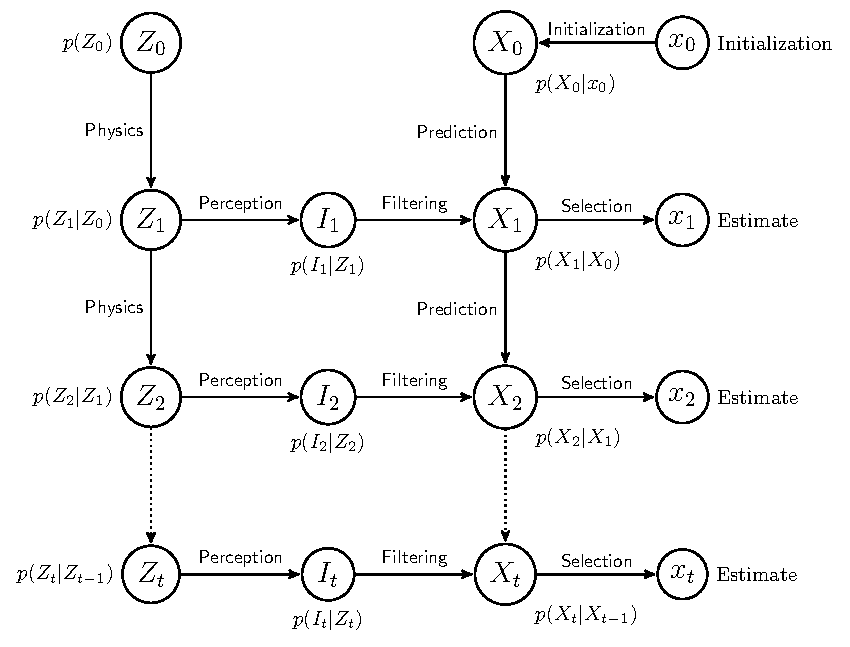
\includegraphics[width=0.8\textwidth]{hmm-pf-graph.pdf}
  \caption{Schematic image of the particle filter alongside a HMM.}
  \label{fig:hmm-graph}
\end{figure}

Figure \ref{fig:hmm-graph} shows the principle of the particle filter
working alongside a hidden Markov model. The following is the core
function of the particle filter:

\begin{quote}
  \emph{The particle filter attempts to approximate the PDF
    $\cprobnext{Z}$ as a set $X_t$ of discrete hypotheses.}
\end{quote}

More particles mean greater accuracy, since the PDF can then be
approximated more closely. However, using many particles increses
computational cost.  Therefore the number of particles is an important
trade-off.  The particle filter employs a few tricks to \emph{filter}
the hypotheses, tending to keep probable ones and throwing improbable
ones away, in order to intelligently reduce the number of particles
needed for a good approximation. The filter works in four steps:

\begin{description}
\item[Prediction] The hypotheses $X_{t-1}$ are updated in the
  \emph{prediction} step to an approximation $\bar{X}_t$ of
  $\cprobnext{Z}$.  This is done by drawing new samples
  $\cprobnext{x}$, for each $x_{t-1}$ in $X_{t-1}$.
\item[Perception] By measuring the state of the system, we gain an
  \emph{observation} $I_t \sim \cprob{I_t}{Z_t}$ of the state $Z_t$.
\item[Filtering] The observation $I_t$ of the system is then used for
  filtering bad hypotheses out of $\bar{X}_t$.  We draw samples $X_t$
  from $\bar{X}_t$ with probabilities given by
  $\cprob{I_t}{\bar{X}_t}$. The result will be a surjection, where
  $X_t$ will be a subset of $\bar{X}_t$ where more probable hypotheses
  appear multiple times.<ref:problem without sigma> For this reason,
  this is also known as the \emph{resampling} step. The set $X_t$ is
  the \emph{belief}, our approximation of $\cprobnext{Z}$.
\item[Selection] Finally, we produce a single hypothesis $x_t$ from
  $X_t$ as our \emph{estimate} of the state $Z_t$. Assuming $X_t$ is a
  good approximation of $\cprobnext{Z}$, and that $\cprobnext{Z}$ is
  unimodal, the means value of $X_t$ is a good estimate since it
  approximates the expectation of $\cprobnext{Z}$.  If $\cprobnext{Z}$
  is multimodal, however, the mean could be a bad estimate since the
  expectation may be very improbable.
\end{description}

The reason why this works is the following theorem, which is Theorem
3.1 in \cite{Hedvig} with some modifications to notation:

\begin{theorem}
  Given the PDFs $\cprobnext{x}$, $\cprob{I_t}{x_t}$ and
  $\cprob{x_{t-1}}{I_{t-1} \wedge \dots \wedge I_0}$, the PDF
  $\cprob{x_t}{I_t \wedge \dots \wedge I_0}$ can be expressed as

\begin{equation}
  \cprob{x_t}{I_t \wedge \dots \wedge I_0} = \kappa \cprob{I_t}{x_t} \int{ \cprobnext{x}\cprob{x_{t-1}}{I_{t-1} \wedge \dots \wedge I_0} \mathrm{d}x_{t-1}},
  \label{thm:pf-grand}
\end{equation}
where $\kappa$ is a normalization constant

For the proof of this, see \cite{Hedvig}.

\end{theorem}

Let's sketch out the connection between this and what we've done so
far. For a more rigorous derivation, see chapter 4 of \cite{ProbRob}.

In this thesis, $\cprob{x_t}{I_t \wedge \dots \wedge I_0}$ is
approximated as the set $X_t$ of hypotheses. Substituting this into
\eqref{thm:pf-grand} and replacing the integral with a sum yields

\begin{equation}
  X_t = \kappa \cprob{I_t}{x_t} \sum { \cprobnext{x} X_{t-1} }.
\end{equation}

Note that this is horrible abuse of notation, but from here we can
take the step to

\begin{equation}
  X_t \sim \cprob{I_t}{x_t} \cprobnext{x}
\end{equation}

\subsection{The Particle Filter algorithm}
\begin{table}
  \begin{codebox}
    \Procname{$\proc{Particle-Filter} (X_{t-1},I_t)$}
    \li $\bar{X}_t \gets \emptyset$
    \li \ForEach $x_{t-1} \in X_{t-1}$
    \li \Do
    \li $x_t \gets \proc{Predict}(x_{t-1})$
    \li $w \gets \proc{Importance}(x_t,I_t)$
    \li Append $\left<x_t, w\right>$ to $\bar{X}_t$
    \End
    \li
    
    \li $X_t \gets \emptyset$
    
    \li \While $\abs{X_t} < \abs{\bar{X}_t}$
    \li \Do
    \li Take $\left<x_t, w\right>$ from $\bar{X}_t$ with probability $\propto w$
    \li Append $x_t$ to $X_t$
    \End
    \li \Return $X_t$
  \end{codebox}
  \caption{The particle filter algorithm.}
  \label{alg:pf}
\end{table}

Table \ref{alg:pf} shows the particle filter algorithm. Note that the
functions \textsc{Predict} and \textsc{Importance} are unspecified -
they are problem specific. They correspond to the PDF $\cprobnext{x}$
and $\cprob{I_t}{x_t}$, respectively.

% We draw a set $\bar{X}_t = \xtmN{x}{t}{i}{N}$ of samples from
% $p$. These samples roughly represent a PDF for the current state
% $x_t$, but we have yet to consider our observation.  Therefore, we
% will create a new PDF weighted by how probable the observation $z_t$
% is. For each $x_t^m$, we let $w_t^m := q\left(z_t |
%   x_t\right)$. This defines a discrete PDF where $x_t^m$ is assumed
% with a probability proportional to $w_t^m$. From this final
% distribution we again draw $N$ samples $X_t$, which will be our
% estimate of the current state.  The elements $x_t^m$ are referred to
% as \emph{particles} and the set $X_t$ as the \emph{belief at time
%   $t$}.

In this thesis, the real $x_{t-1}$ is not known. Rather $x_{t-1}$ is
estimated with a set $X_{t-1}$ of $N$ particles.

\section{Visual Cues}

The biggest problem with computer vision is that computers do not have
vision, only a data input device in the form of a camera.

A \emph{visual cue} is an image transformation $\phi$ that extracts
some property of the image, such as intensity, edges or ridges.

<ref to machine vs biological comparison study>

<image showing the use of $\phi$>

Assuming that a whisker has one fix point of origin<ref:analysis(this is not
the case really)> we have the boundary condition $whisker(0)=0$

"There are many metrics by which a model may be assessed." - Encyclopedia
(>model evaluation)

"
==Model selection
Model selection is the process of choosing an appropriate mathematical model
from a class of models.
" - Encyclopedia 
The class being all functions with f(0)=0,contioiuns(or stronger?) and finite number of parameters




\begin{theorem} %TODO svagare?
    \label{thm:response_max}
    Let $f$ be a positive Riemann function with compact support, then
    \begin{equation}
      \argmax{\bar{e}}
      \left(
        \sum\limits_{\Omega}{f(\bar{x})f(\bar{x}-\bar{e})}
      \right)
      =0
    \end{equation}
\end{theorem}
\begin{proof}
  Firstly define the window function as
  \begin{equation}
    W_a^b(x)=
    \begin{cases}
      0,~& x<a\\
      1,~& a \leq x \leq b\\
      0,~& x>b
    \end{cases}
  \end{equation}
  Multiplication
  \begin{equation}
    (W_a^bW_c^d)(x)=W_{\max(a,c)}^{\min(b,d)}(x)
  \end{equation}
  Translation
  \begin{equation}
    W_a^b(x-e)=W_{a+e}^{b+e}(x)
  \end{equation}
  Integration
  \begin{equation}
    \label{eq:int_window}
    \sum{W_a^b(x)dx}=\Theta(b-a)
  \end{equation}
  
  \begin{equation}
    \begin{array}{c}
      
      \argmax{e}\left(
        \sum
        {
          W_a^b(x)W_a^b(x-e)
        }
      \right)
      =\\
      \argmax{e}\left(
        \sum
        {
          W_a^b(x)W_
          {
            a+e
          }
          ^
          {
            b+e
          }
          (x)
        }
      \right)
      =\\
      \argmax{e}\left(
        \sum
        {
          W_
          {
            \max(a,a+e)
          }^
          {
            \min(b,b+e)
          }
          (x)
        }
      \right)
      =\\
      \argmax{e}\left(
        \Theta(\min(b,b+e)-\max(a,a+e))
      \right)
      =\\
      % \left\{\text{
      %     max the min and min the max at the same time
      %   }
      % \right\}=\\
      0
    \end{array}
  \end{equation}
  
  This trivially holds with superposition of windows, since all
  windows will scale and translate the same way.  With a finite
  support $e=0$ is the only solution. Additionaly this also hold in
  higher finite dimensions since we can just repeat the process for
  one dimension at a time.
    
  All riemann functions can be written as a superposition of windows
  like this
  \begin{equation}
    f(x)=\sum{c_iW_{a_i}^{b_i}(x)}
  \end{equation}
  
  $\therefore$ Each riemann function $f$ with finite support will have a $e=0\qed$
  
\end{proof}

=============================

\subsubsection{ Theoretical evalutaion (formal methods)}

============================

============== MODELS =================

One possible model is to borrow the model for beam under small
deformations from the theory of strength of materials, after all the
whisker is a beam but we dont have small deformations at all but we
assume that the model will approximatly hold ony way.


